%% Seminar deck: Does the term premium pay for the duration? (preprint, 2026)
%% 13 slides, yieldcartography house theme, academic-seminar register.
%% Built from the Research Square v1 preprint (89-bond panel, 2006-12-29 to
%% 2026-05-15). No venue disclosed.
\documentclass[aspectratio=169,11pt]{beamer}
\usepackage{beamerthemeyc}
\renewcommand{\deckfootertitle}{Dec (2026) · Does the term premium pay for the duration? · preprint}

\begin{document}

% 1 ---------------------------------------------------------------------------
\begin{frame}[plain]
  \vspace{2mm}
  {\ttfamily\scriptsize\color{ycmuted}SEMINAR DECK · YIELDCARTOGRAPHY.COM}\\[-0.3em]
  {\color{ycrule}\rule{\textwidth}{0.5pt}}
  \vspace{4mm}

  {\fontsize{19}{23}\selectfont\bfseries\color{ycink}Does the term premium\\pay for the duration?\par}
  \vspace{2mm}
  {\normalsize\color{ycmuted}Evidence from Polish sovereigns.\par}
  \vspace{6mm}
  {\small\bfseries Marcin Dec\par}
  {\footnotesize\color{ycmuted}Kozminski University \& FAME|GRAPE, Warsaw\par}
  \vspace{3mm}
  {\ttfamily\scriptsize\color{ycaccent}Research Square preprint v1, June 2026 · doi:10.21203/rs.3.rs-9849665/v1 · under peer review\par}
  \vfill
  \raisebox{-1mm}{
\includegraphics[height=6mm]{kozminski_logo.png}}\hspace{5mm}
  \raisebox{-1mm}{
\includegraphics[height=6mm]{grape_logo.png}}\hspace{5mm}
  \raisebox{-1mm}{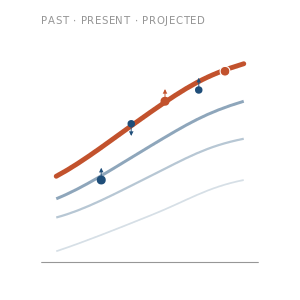
\includegraphics[height=6mm]{yc_logo.png}}
  \hfill{\ttfamily\scriptsize\color{ycmuted}NCN Preludium UMO-2020/37/N/HS4/02202}
\end{frame}

% 2 ---------------------------------------------------------------------------
\begin{frame}{Motivation}
  \kicker{Ex-ante premia versus realised attribution}
  \begin{itemize}
    \item On the Polish curve the ex-ante term premium is positive on average:
          roughly $+105$ bp at the 10-year tenor under ACM with the BRW
          small-sample bias correction, and positive on the large majority of
          days. The textbook implication is that a duration position over
          rolling short-term cash earns this premium.
    \item The empirical question is the realised counterpart: of the 4.14\%
          compound annual return the published TBSP index delivered over
          nineteen years, \alert{what share is attributable to term-premium
          realisation}, and what share to coupon accrual, reinvestment and
          roll-down?
    \item The benchmark cash rate throughout is the NBP reference rate, a
          proxy for the upper envelope of retail deposit rates.
  \end{itemize}
\end{frame}

% 3 ---------------------------------------------------------------------------
\begin{frame}{A seven-component identity for the quarterly index return}
  \kicker{Decomposition}
  \small Each quarter's TBSP log-return is partitioned in closed form:
  \[ r_t \;=\; \underbrace{CC_t + RP_t + RD_t}_{\text{CarryRoll}}
     \;+\; \underbrace{ERC_t + TPC_t}_{\text{CurveMove}}
     \;+\; Cnvx_t \;+\; Res_t \]
  \begin{itemize}
    \item $CC$ coupon accrual, $RP$ reinvestment proceeds, $RD$ clean-price
          roll-down along an unchanged curve: the return to an unchanged state
          of the world.
    \item $ERC$ and $TPC$: revaluation from the expected-rate and term-premium
          legs of the ACM--BRW decomposition of the fitted zero curve.
    \item $Cnvx$ second-order convexity; $Res$ the closure residual. The sum
          reproduces the published index by construction; no estimation enters
          the partition.
    \item The split of CurveMove rests on the fitted-curve decomposition
          \( y_t(\tau) = y^{rf}_t(\tau) + tp_t(\tau) \): the ACM--BRW
          expected-rate leg and term-premium leg of the LW-NSS zero curve,
          each revalued separately.
  \end{itemize}
\end{frame}

% 4 ---------------------------------------------------------------------------
\begin{frame}{Data and replication quality}
  \kicker{The panel}
  \begin{itemize}
    \item Published Treasury BondSpot Poland (TBSP) index, 2006-12-29 to
          2026-05-15, 80 quarter-end snapshots, replicated bond by bond on an
          89-bond BondSpot panel with daily LW-NSS zero curves.
    \item Closure residual: $+20$ bp cumulative over the full sample.
          Tracking gap against the published index: $-106$ bp cumulative
          ($-5.4$ bp per year). Both are an order of magnitude below the
          components being attributed.
  \end{itemize}
\end{frame}

% 5 ---------------------------------------------------------------------------
\begin{frame}{Result 1: the carry-and-roll bloc}
  \kicker{Cumulative attribution, 2006-12-29 to 2026-05-15}
  \begin{itemize}
    \item CarryRoll ($CC+RP+RD$) cumulates to $+8{,}010$ bp, $+413$ bp per
          year of sample, against the $+7{,}866$ bp ($+405$ bp per year)
          delivered by the published index.
    \item Within the bloc, coupon accrual contributes $+7{,}604.9$ bp,
          roll-down $+361.4$ bp and reinvestment $+43.7$ bp: the income bloc
          alone accounts for essentially the entire realised return.
    \item Convexity adds a further $+278.8$ bp ($+14.4$ per year), a
          second-order but persistent positive term.
  \end{itemize}
\end{frame}

% 6 ---------------------------------------------------------------------------
\begin{frame}{The full attribution, per year of sample}
  \kicker{Cumulative contribution / sample length}
  \begin{center}
  \begin{tikzpicture}[x=0.0225cm,y=0.62cm]
    \draw[ycmuted,line width=0.5pt] (0,-0.4) -- (0,7.6);
    \foreach [count=\i] \lab/\v/\c in {
        Coupon accrual/391.7/ycaccent,
        Roll-down/18.6/ycaccent!60,
        Convexity/14.4/ycrule,
        Reinvestment/2.3/ycrule,
        Residual/1.0/ycrule,
        Expected-rate change/-4.8/ycsalmon!60,
        Tracking gap/-5.4/ycrule,
        Term-premium change/-12.6/ycsalmon}{
      \pgfmathsetmacro{\yy}{7.6-\i}
      \fill[\c] (0,\yy) rectangle (\v*0.55,\yy+0.42);
      \node[left=3pt,font=\scriptsize,text=ycink,anchor=east] at (0,\yy+0.21) {\lab};
      \node[font=\scriptsize\bfseries,text=ycink,anchor=west] at ({max(\v*0.55,0)+3},\yy+0.21)
        {\pgfmathparse{\v>0?"+":""}\pgfmathresult\v};
    }
    \node[below,font=\tiny\itshape,text=ycmuted] at (60,-0.8) {bp per year};
  \end{tikzpicture}
  \end{center}
  \footnotesize\color{ycmuted} Components sum to the published TBSP log-return,
  $+405$ bp per year. Coupon accrual exceeds all other components combined.
\end{frame}

% 7 ---------------------------------------------------------------------------
\begin{frame}{Result 2: full-sample inference on the curve-move bloc}
  \kicker{HAC tests and bootstrap intervals}
  \begin{itemize}
    \item $ERC+TPC$ cumulates to $-337$ bp over the sample ($-17$ bp per
          year), largely the unreversed portion of the 2022 tightening-cycle
          revaluation.
    \item The full-sample tests are uninformative: the mean realised $TPC$ of
          $-3.1$ bp per quarter has HAC $p=0.83$, with a bootstrap confidence
          interval on the cumulative of $[-2{,}534,\,+1{,}776]$ bp; the
          TBSP-versus-cash excess of $+17.6$ bp per quarter has $p=0.55$.
          Both intervals bracket zero.
    \item The tests: with $e_t = r^{TBSP}_t - r^{cash}_t$ the null is
          $H_0\!: \mathbb{E}[e_t]=0$, assessed by
          \( t = \bar e \,/\, \sqrt{\widehat{V}_{NW}/T} \) and by bootstrap
          intervals on cumulative sums; the same construction applies to the
          $TPC$ series.
    \item The width of the intervals reflects the concentration of the
          series' variance in a single regime episode; conditioning on that
          episode is the natural next step.
  \end{itemize}
\end{frame}

% 8 ---------------------------------------------------------------------------
\begin{frame}{The 2021Q4--2022Q3 tightening episode}
  \kicker{One episode dominates the sample moments}
  \begin{itemize}
    \item Four quarters contribute $-962$ bp of cumulative term-premium
          change: four times the full sample's net $-245$ bp.
    \item The index fell from 2{,}175 to 1{,}703 peak-to-trough, a $-21.7\%$
          drawdown, only partially reversed after 2023.
    \item Treating these quarters as part of a homogeneous sample conflates a
          rare regime realisation with the unconditional distribution; the
          paper conditions on the episode explicitly; dummy-variable
          specifications are reported as robustness.
  \end{itemize}
\end{frame}

% 9 ---------------------------------------------------------------------------
\begin{frame}{Result 3: the conditional excess return}
  \kicker{Excluding the four episode quarters}
  \begin{itemize}
    \item On the 74-quarter sub-sample the mean TBSP-versus-rolling-cash
          excess is $+46.5$ bp per quarter, HAC $p=0.003$, with a cumulative
          bootstrap confidence interval of $[+1{,}217,\,+5{,}534]$ bp.
    \item The full-sample counterpart is $+17.6$ bp per quarter
          ($+1{,}354$ bp cumulative), $p=0.55$: the four episode quarters move
          the point estimate by a factor of 2.6 and inflate the variance
          enough to remove significance.
    \item The excess over cash is positive on 74 of the 78 quarter-ends of the
          full sample.
  \end{itemize}
\end{frame}

% 10 --------------------------------------------------------------------------
\begin{frame}{Interpretation}
  \kicker{Reconciling ex-ante and realised premia}
  \small
  \begin{itemize}
    \item A positive ex-ante term premium coexists with a realised
          term-premium contribution indistinguishable from zero because
          realisation risk is concentrated in rare, persistent regime
          episodes; unconditional sample means therefore converge slowly.
    \item A TBSP-tracking exposure is characterised as a carry position
          between the term spread and the policy rate bearing low-frequency
          regime risk; the ex-ante premium is realised only conditionally on
          the regime path.
    \item The characterisation reproduces the observed moments: the long-run
          excess over cash, the modest trailing information ratio (0.21), and
          the depth of the 2022 drawdown.
  \end{itemize}
\end{frame}

% 11 --------------------------------------------------------------------------
\begin{frame}{Data and econometrics}
  \kicker{Specification summary}
  \small
  \begin{itemize}
    \item \textbf{Identity.} Closed-form seven-component partition of the
          quarterly log-return of a coupon-bearing bond, aggregated with
          published TBSP weights; derivation and closure properties in the
          paper's appendix.
    \item \textbf{Curves.} Daily LW-NSS zero curves; expected-rate and
          term-premium legs from ACM with the BRW small-sample bias
          correction.
    \item \textbf{Inference.} Newey--West (HAC) tests on quarterly means and
          bootstrap confidence intervals on cumulative contributions; the
          regime episode is handled by explicit conditioning.
    \item \textbf{Verification.} The closure residual and the tracking gap
          against the published index are reported explicitly: $+20$ bp and
          $-106$ bp cumulative respectively.
  \end{itemize}
\end{frame}

% 12 --------------------------------------------------------------------------
\begin{frame}{Companion data and replication}
  \kicker{yieldcartography.com}
  \begin{itemize}
    \item The identity runs on each quarter as it closes: index-level cards and
          a per-bond explorer at
          \textcolor{ycaccent}{\ttfamily yieldcartography.com/total-return}.
    \item The ACM--BRW expected-rate and term-premium legs update daily on
          \textcolor{ycaccent}{\ttfamily /term-premia/}; the current
          quarter-to-date decomposition is carried on the cockpit.
    \item Underlying CSVs are downloadable from the dashboards.
  \end{itemize}
\end{frame}

% 13 --------------------------------------------------------------------------
\begin{frame}[plain]
  \vspace{12mm}
  {\fontsize{27}{31}\selectfont\bfseries\color{ycink}Thank you.\par}
  \vspace{6mm}
  {\normalsize\color{ycink}Marcin Dec\par}
  {\small\color{ycmuted}Kozminski University \& FAME|GRAPE, Warsaw\\
   mdec@kozminski.edu.pl · ORCID 0000-0002-6220-8267\par}
  \vspace{5mm}
  {\ttfamily\footnotesize\color{ycaccent}%
   Dec, M. (2026). Does the term premium pay for the duration?\\
   Evidence from Polish sovereigns. Research Square preprint v1.\\
   doi:10.21203/rs.3.rs-9849665/v1 · under peer review\par}
  \vspace{5mm}
  {\ttfamily\scriptsize\color{ycmuted}Research supported by the National
   Science Centre, Poland · Preludium UMO-2020/37/N/HS4/02202\par}
  \vfill
  \raisebox{-1mm}{
\includegraphics[height=6mm]{kozminski_logo.png}}\hspace{5mm}
  \raisebox{-1mm}{
\includegraphics[height=6mm]{grape_logo.png}}\hspace{5mm}
  \raisebox{-1mm}{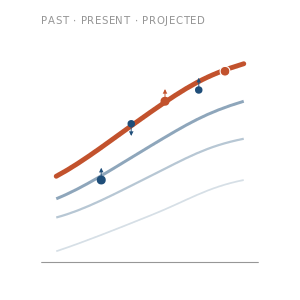
\includegraphics[height=6mm]{yc_logo.png}}
  \hfill{\ttfamily\scriptsize\color{ycmuted}yieldcartography.com/slides/duration/}
\end{frame}

\end{document}
